\documentclass[svgnames,11pt]{beamer}
\input{/home/tof/Documents/Cozy/latex-include/preambule_commun.tex}
\input{/home/tof/Documents/Cozy/latex-include/preambule_beamer.tex}
%\usepackage{pgfpages} \setbeameroption{show notes on second screen=left}
\author[]{Christophe Viroulaud}
\title{Saut en longueur\\les tableaux}
\date{\framebox{\textbf{DonRep 07}}}
%\logo{}
\institute{Première - NSI}
%DODO parcours séquentiel trop dur (à faire après/pendant Algo parcours séquentiel)
\begin{document}
\begin{frame}
    \titlepage
\end{frame}
\begin{frame}
    \frametitle{}

    La finale du saut en longueur des championnats du monde de 1991 est considérée comme l'un des meilleurs concours de l'histoire de la discipline. Elle oppose principalement Carl Lewis, invaincu depuis 10 ans, et Mike Powell, son plus grand rival.
    \begin{center}
        \centering
        \includegraphics[width=8cm]{ressources/lewis.jpg}
        \captionof{figure}{Carl Lewis}
        \label{IMG}
    \end{center}

\end{frame}
\begin{frame}
    \frametitle{}

    Chaque athlète effectue six sauts. Les mesures sont stockées au fur et à mesure du concours. La meilleure performance consacre le vainqueur.

    \begin{framed}\centering
        Comment stocker une série de données \textbf{modifiables} dans un programme?
    \end{framed}

\end{frame}
\section{Les tableaux}
\subsection{Présentation}
\begin{frame}[fragile]
    \frametitle{}

    \begin{aretenir}[]
        Un tableau est une séquence \textbf{ordonnée} d'éléments \textbf{de même type}. Un tableau est \textbf{modifiable}.
    \end{aretenir}
    \begin{center}
        \begin{lstlisting}[language=Python , basicstyle=\ttfamily\small, xleftmargin=2em, xrightmargin=2em]
un_tableau = [3, 6, 1, 7]
\end{lstlisting}
        \captionof{code}{Construire un tableau en Python: les crochets}
        \label{CODE}
    \end{center}
\end{frame}
\begin{frame}
    \frametitle{}


    \begin{aretenir}[Remarque]
        En Python, on utilise souvent le terme \textbf{\texttt{list}} pour évoquer un tableau.
    \end{aretenir}

\end{frame}
\begin{frame}
    \frametitle{}
    On se propose de suivre le concours au fur et à mesure des sauts et d'enregistrer les performances des athlètes après chaque tentative.
    \begin{activite}
        \begin{enumerate}
            \item Construire deux tableaux \textbf{\texttt{lewis}} et \textbf{\texttt{powell}} contenant chacun six zéros.
            \item Afficher les deux tableaux avec l'instruction \textbf{\texttt{print}}.
        \end{enumerate}
    \end{activite}

\end{frame}
\begin{frame}[fragile]
    \frametitle{Correction}

    \begin{center}
        \begin{lstlisting}[language=Python , basicstyle=\ttfamily\small, xleftmargin=2em, xrightmargin=2em]
lewis = [0., 0., 0., 0., 0., 0.]
powell = [0., 0., 0., 0., 0., 0.]
print("Carl Lewis", lewis)
print("Mike Powell", powell)
\end{lstlisting}
        \captionof{code}{Début du concours}
        \label{CODE}
    \end{center}
    \begin{aretenir}[Remarque]
        Les données sont des nombres flottants.
    \end{aretenir}
\end{frame}
\subsection{Modifier un élément du tableau}
\begin{frame}
    \frametitle{Modifier un élément du tableau}
    \begin{aretenir}[]
        Chaque élément est repérable par sa position dans le tableau. La numérotation commence à zéro.
    \end{aretenir}
    \begin{center}
        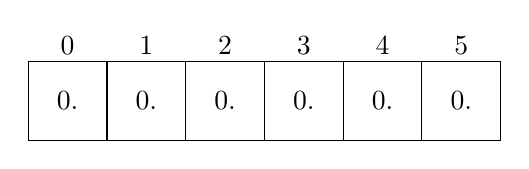
\begin{tikzpicture}
            \draw (0,0) grid (6,1);
            \foreach \x in {0,1,...,5}{
                    \node at (0.5+\x, 1.2) {\x};
                    \node at (0.5+\x, .5) {0.};
                }
        \end{tikzpicture}
    \end{center}

\end{frame}
\begin{frame}[fragile]
    \frametitle{}

    \begin{center}
        \begin{lstlisting}[language=Python , basicstyle=\ttfamily\small, xleftmargin=2em, xrightmargin=2em]
>>> lewis[0]
0.0
\end{lstlisting}
        \captionof{code}{Lecture d'un élément}
        \label{CODE}
    \end{center}
    Lewis entame la compétition de manière exceptionnelle avec un saut à 8,68 m. Powell ne saute qu'à 7,85m.
    \begin{center}
        \begin{lstlisting}[language=Python , basicstyle=\ttfamily\small, xleftmargin=2em, xrightmargin=2em]
lewis[0] = 8.68
powell[0] = 7.85
\end{lstlisting}
        \captionof{code}{Écriture d'un élément}
        \label{CODE}
    \end{center}
\end{frame}
\begin{frame}[fragile]
    \frametitle{}

    \begin{lstlisting}[language=Python , basicstyle=\ttfamily\small, xleftmargin=2em, xrightmargin=2em]
lewis = [0., 0., 0., 0., 0., 0.]
powell = [0., 0., 0., 0., 0., 0.]
print("Carl Lewis", lewis)
print("Mike Powell", powell)

# 1er saut
lewis[0] = 8.68
powell[0] = 7.85
print("Carl Lewis", lewis)
print("Mike Powell", powell)
\end{lstlisting}
    \begin{center}
        \begin{lstlisting}[language=Python , basicstyle=\ttfamily\small, xleftmargin=2em, xrightmargin=2em]
Carl Lewis [0.0, 0.0, 0.0, 0.0, 0.0, 0.0]
Mike Powell [0.0, 0.0, 0.0, 0.0, 0.0, 0.0]
Carl Lewis [8.68, 0.0, 0.0, 0.0, 0.0, 0.0]
Mike Powell [7.85, 0.0, 0.0, 0.0, 0.0, 0.0]
\end{lstlisting}
        \captionof{code}{Affichage dans la console}
        \label{CODE}
    \end{center}
\end{frame}
\begin{frame}
    \frametitle{}

    \begin{activite}
        Poursuivre le programme au fur et à mesure du concours.
    \end{activite}

\end{frame}
\begin{frame}
    \frametitle{}

    Au deuxième saut, Powell se rapproche de Lewis. Malgré son piétinement avant la planche, il réalise 8,54 m. Carl Lewis mord.

\end{frame}
\begin{frame}[fragile]
    \frametitle{}

    \begin{lstlisting}[language=Python , basicstyle=\ttfamily\small, xleftmargin=2em, xrightmargin=2em]
# 2eme saut
lewis[1] = 0.
powell[1] = 8.54
print("Carl Lewis", lewis)
print("Mike Powell", powell)
\end{lstlisting}

\end{frame}

\begin{frame}
    \frametitle{}

    Lors de son saut, Powell touche le sable avec ses fesses, limitant son saut à 8,29 m. Puis Lewis saute, aidé par le vent, à 8,83 m.

\end{frame}
\begin{frame}[fragile]
    \frametitle{}

    \begin{lstlisting}[language=Python , basicstyle=\ttfamily\small, xleftmargin=2em, xrightmargin=2em]
# 3eme saut
lewis[2] = 8.83
powell[2] = 8.29
print("Carl Lewis", lewis)
print("Mike Powell", powell)
\end{lstlisting}

\end{frame}

\begin{frame}
    \frametitle{}

    Powell commet à nouveau une faute, son saut non mesuré est estimé à 8,80 m. Il va lui-même vérifier la griffe sur la plasticine. Lewis répond de nouveau avec un saut encore plus loin : bien que l'anémomètre indique que le vent est trop favorable pour constituer un record homologué, le saut est toutefois validé pour le concours à 8,91 m.

\end{frame}
\begin{frame}[fragile]
    \frametitle{}

    \begin{lstlisting}[language=Python , basicstyle=\ttfamily\small, xleftmargin=2em, xrightmargin=2em]
# 4eme saut
lewis[3] = 8.91
powell[3] = 0.
print("Carl Lewis", lewis)
print("Mike Powell", powell)
\end{lstlisting}

\end{frame}
\begin{frame}
    \frametitle{}

    Au cinquième tour, Powell donne également toute la mesure de son talent. Il effectue cette fois un saut valide avec un vent dans le dos de 0,3 m/s, ce qui reste dans la limite autorisée pour l'homologation d'un record. Après quelques secondes d'attente, le public et Powell explosent en découvrant la distance, 8,95 m, un nouveau record du monde.\\
    Il reste deux essais à Lewis pour battre Powell. Il saute à 8,87 m avec un vent de face, un nouveau record personnel en conditions autorisées.

\end{frame}
\begin{frame}[fragile]
    \frametitle{}

    \begin{lstlisting}[language=Python , basicstyle=\ttfamily\small, xleftmargin=2em, xrightmargin=2em]
# 5eme saut
lewis[4] = 8.87
powell[4] = 8.95
print("Carl Lewis", lewis)
print("Mike Powell", powell)
\end{lstlisting}

\end{frame}
\begin{frame}
    \frametitle{}

    Le dernier saut de Powell est mordu. Il se rhabille et prie en attendant le sixième essai de Lewis. Le saut est mesuré à 8,84 m. Powell est champion du monde et nouveau recordman de la discipline.

\end{frame}
\begin{frame}[fragile]
    \frametitle{}

    \begin{lstlisting}[language=Python , basicstyle=\ttfamily\small, xleftmargin=2em, xrightmargin=2em]
# 6eme saut
lewis[5] = 8.84
powell[5] = 0.
print("Carl Lewis", lewis)
print("Mike Powell", powell)
\end{lstlisting}

\end{frame}
\subsection{Propriétés d'un tableau}
\begin{frame}
    \frametitle{Propriétés d'un tableau}

    \begin{aretenir}[]
        Un tableau est \textbf{mutable}. On utilise la structure à crochets pour lire ou modifier un élément d'un tableau.
    \end{aretenir}

\end{frame}
\begin{frame}[fragile]
    \frametitle{}

    \begin{aretenir}[]
        La fonction \textbf{\texttt{len}} renvoie la taille d'un tableau.
    \end{aretenir}


    \begin{lstlisting}[language=Python , basicstyle=\ttfamily\small, xleftmargin=2em, xrightmargin=2em]
>>> len(lewis)
6
\end{lstlisting}
\end{frame}
\begin{frame}
    \frametitle{}

    \begin{activite}
        \begin{enumerate}
            \item Écrire la fonction \textbf{\texttt{meilleure\_perf(tab: list) $\rightarrow$ float}} qui renvoie la plus grande valeur du tableau.
            \item Écrire la fonction \textbf{\texttt{moyenne(tab: list) $\rightarrow$ float}} qui renvoie la moyenne des performances. Les essais manqués ne seront pas pris en compte dans le calcul de la moyenne.
        \end{enumerate}
    \end{activite}

\end{frame}
\begin{frame}[fragile]
    \frametitle{Correction}

    \begin{lstlisting}[language=Python , basicstyle=\ttfamily\small, xleftmargin=2em, xrightmargin=2em]
def meilleure_perf(tab: list) -> float:
    """
    renvoie la plus grande valeur du tableau
    """
    meilleure = 0
    for perf in tab:
        if perf > meilleure:
            meilleure = perf

    return meilleure
\end{lstlisting}
    \begin{center}
        \begin{lstlisting}[language=Python , basicstyle=\ttfamily\small, xleftmargin=2em, xrightmargin=2em]
>>> meilleure_perf(powell)
8.95
\end{lstlisting}
        \captionof{code}{Appel de la fonction}
        \label{CODE}
    \end{center}
\end{frame}
\begin{frame}[fragile]

    \begin{lstlisting}[language=Python , basicstyle=\ttfamily\small, xleftmargin=2em, xrightmargin=2em]
def moyenne(tab: list) -> float:
    """
    calcule la moyenne des valeurs du tableau
    Les 0 ne sont pas pris en compte.
    """
    somme = 0
    nb_sauts = 0
    for perf in tab:
        if perf > 0: # sauts ratés pas pris
            somme += perf
            nb_sauts += 1

    return somme/nb_sauts
\end{lstlisting}
    \begin{center}
        \begin{lstlisting}[language=Python , basicstyle=\ttfamily\small, xleftmargin=2em, xrightmargin=2em]
>>> moyenne(powell)
8.407499999999999
\end{lstlisting}
        \captionof{code}{Appel de la fonction}
        \label{CODE}
    \end{center}
\end{frame}
\begin{frame}[fragile]
    \frametitle{}
    \begin{center}
        \begin{lstlisting}[language=Python , basicstyle=\ttfamily\small, xleftmargin=2em, xrightmargin=2em]
def moyenne(tab: list) -> float:
    """
    calcule la moyenne des valeurs du tableau
    Les 0 ne sont pas pris en compte.
    """
    somme = 0
    nb_sauts = 0
    for perf in tab:
        if perf > 0: # sauts ratés pas pris
            somme += perf
            nb_sauts += 1
    
    # si tous les sauts sont ratés
    if nb_sauts == 0:
        return 0
    else:
        return somme/nb_sauts
\end{lstlisting}
        \captionof{code}{Prise en compte des erreurs}
        \label{CODE}
    \end{center}

\end{frame}
\section{Utiliser un tableau dans une fonction}
\begin{frame}[fragile]
    \frametitle{Utiliser un tableau dans une fonction}
    Rappelons le déroulement de l'exécution d'une fonction:
    \begin{lstlisting}[language=Python , basicstyle=\ttfamily\small, xleftmargin=2em, xrightmargin=2em]
def cube(x: int) -> int:
    resultat = x**3
    return resultat

a = 5
b = cube(a)
\end{lstlisting}
    \begin{center}
        \begin{tikzpicture}[scale=0.8,transform shape]
            \node[draw] (5) at (-3, 4) {5};
            \node at(-3,3.5) {a};
            \node[draw] (125) at (-3, 2) {};
            \node at(-3,1.5) {b};
            \draw (0,0) -- (4,0) -- (4,3) -- (0,3) -- cycle;
            \node[anchor=west] at (0,2.7) {cube};
            \draw[->,>=latex] (5) edge[bend left] (1.5, 2.5);
        \end{tikzpicture}
        \captionof{figure}{\centering Une copie du \textbf{contenu} de la variable \textbf{\texttt{a}} est passée dans la fonction.}
    \end{center}

\end{frame}
\begin{frame}
    \frametitle{}

    \begin{center}
        \begin{tikzpicture}
            \node[draw] (5) at (-3, 4) {5};
            \node at(-3,3.5) {a};
            \node[draw] (125) at (-3, 2) {};
            \node at(-3,1.5) {b};
            \draw (0,0) -- (4,0) -- (4,3) -- (0,3) -- cycle;
            \node[anchor=west] at (0,2.7) {cube};
            \node at(1,2) {x = 5};
            \node at (1.7,1) {resultat = 125};
        \end{tikzpicture}
        \captionof{figure}{\centering Le \textbf{paramètre} \textbf{\texttt{x}} contient la valeur 5.}
    \end{center}


\end{frame}
\begin{frame}
    \frametitle{}

    \begin{center}
        \begin{tikzpicture}
            \node[draw] (5) at (-3, 4) {5};
            \node at(-3,3.5) {a};
            \node[draw] (125) at (-3, 2) {125};
            \node at(-3,1.5) {b};
            \draw (0,0) -- (4,0) -- (4,3) -- (0,3) -- cycle;
            \node[anchor=west] at (0,2.7) {cube};
            \node at(1,2) {x = 5};
            \node at (1.7,1) {resultat = 125};
            \draw[->,>=latex] (2.5,0.8) edge[bend left] (125);
        \end{tikzpicture}
        \captionof{figure}{\centering Le \textbf{contenu} de \textbf{\texttt{resultat}} est renvoyé à \textbf{\texttt{b}}.}
    \end{center}

\end{frame}
\begin{frame}
    \frametitle{}

    \begin{aretenir}[]
        Les types \emph{de bases} ne sont pas \textbf{mutables}. On passe une copie de la valeur dans une fonction.
    \end{aretenir}

\end{frame}
\begin{frame}[fragile]
    \frametitle{}

    \begin{lstlisting}[language=Python , basicstyle=\ttfamily\small, xleftmargin=2em, xrightmargin=2em]
def ma_fonction(t: list) -> None:
    t[0] = 19

tab = [3, 4, 5]
ma_fonction(tab)
\end{lstlisting}
    \begin{activite}
        Écrire le code précédent dans Pythontutor et observer l'exécution de la fonction.
    \end{activite}
\end{frame}
\begin{frame}
    \frametitle{}


    \begin{center}
        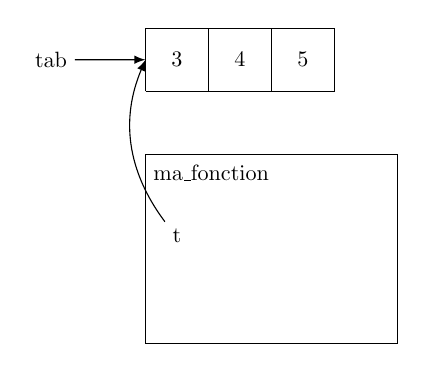
\begin{tikzpicture}[scale=0.8,transform shape]
            \draw (0,4) grid (3,5);
            \foreach \x in {3,4,5}{
                    \node at (-2.5+\x, 4.5) {\x};
                }
            \node (tab) at(-1.5,4.5) {tab};
            \draw (0,0) -- (4,0) -- (4,3) -- (0,3) -- cycle;
            \node[anchor=west] at (0,2.7) {ma\_fonction};
            \node (t) at(0.5,1.7) {t};
            \draw[->,>=latex] (tab) to (0,4.5);
            \draw[->,>=latex] (t) edge[bend left] (0,4.5);
        \end{tikzpicture}
        \captionof{figure}{\centering Les variables \textbf{\texttt{tab}} et \textbf{\texttt{t}} référencent le même tableau.}
    \end{center}
    \begin{aretenir}[]
        Un tableau est une donnée \textbf{mutable}. On passe une \textbf{référence} à ce tableau dans la fonction.
    \end{aretenir}
\end{frame}
\end{document}
